\section{Durchführung}
\label{sec:Durchführung}

\subsection{Untersuchung eines Acrylblocks mit dem A-Scan und Untersuchung des Auflösungsvermögens} \label{sec:1}
In diesem Versuchsteil wird zunächst ein Acrylblock vermessen. In diesem befinden sich Störstellen, wie in Abbildung \ref{fig:block} zu sehen ist.
\begin{figure}[H]
  \centering
  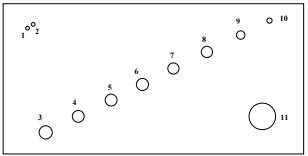
\includegraphics{Text/Bilder/Block.PNG}
  \caption{Schematische 2D-darstellung des zu vermessenden Blocks \cite[5]{sample}}
  \label{fig:block}
\end{figure}
Daraufhin wird die Lage der Störstellen mithilfe des Impuls-Echo-Verfahrens bestimmt. Dazu wird der Block zunächst auf ein Papiertuch gestellt und daraufhin mit einer
$\SI{2}{\mega\hertz}$-Sonde gekoppelt. Als Kopplungsmittel wird Wasser verwendet.
Mit einem A-Scan wird dann von mehreren Seiten die Tiefe der Störstellen gemessen.
\newline
Zur Untersuchung des Auflösungsvermögens werden die Fehlstellen $1$ und $2$ aus Abbildung \ref{fig:block} mithilfe des A-Scans genauer untersucht.
Dazu werden sie zunächst mit einer $\SI{2}{\mega\hertz}$ gemessen. Daraufhin wird der Vorgang mit sowohl mit einer $\SI{1}{\mega\hertz}$-Sonde als auch mit einer $\SI{4}{\mega\hertz}$-Sonde wiederholt

\subsection{Untersuchung eines Acrylblocks mit dem B-Scan}
in diesem Versuchsteil wird der Aufbau aus Kapitel \ref{sec:1} verwendet. Jedoch wird dieses mal ein B-Scan durchgeführt, indem die gekoppelte Sonde mit möglichst konstanter Geschwindigkeit
über den Acrylblock geführt wird. Daraufhin wird der Acrylblock so gedreht, dass die vorher unten liegende Seite oben liegt und die Messung erneut durchgeführt.

\subsection{Untersuchung eines Herzmodells mit dem TM-Scan}
Zunächst wird das Herzmodell zu einem Drittel mit Wasser befüllt. Daraufhin wird eine $\SI{2}{\mega\hertz}$ Sonde so positioniert, dass diese gerade das Wasser berührt.
Daraufhin wird mithilfe eines Gummiballs die Membran periodisch gewölbt und ein TM-Scan durchgeführt.
